\documentclass[Main.tex]{subfiles} 
\begin{document}

\subsection{Sprint 5}
I sprint 5 blev programmet samlet.
Dette var en l�ngerevarende proces, som prim�rt bestod af, at samle de forskellige mindre projekter og pakker, som udgjorde det store projekt.
\\
\begin{wrapfigure}{r}{0.6\textwidth}
	\vspace{-20pt}
    \centering
	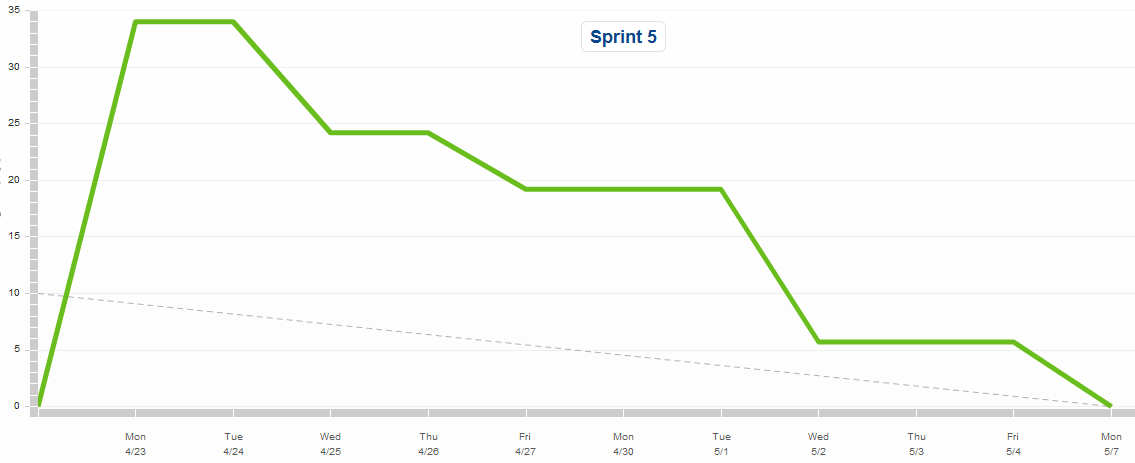
\includegraphics[scale=0.25]{Billeder/Sprint5_burn.png}
    \vspace{-20pt}
	\caption{Burndown chart for sprint 5}
	\vspace{-10pt}
  \label{fig:sprint5}
\end{wrapfigure}
Med de funktionelle komponenter samlet, blev GUI'en omskrevet via MVVM-m�nstret\footnote{\url{http://en.wikipedia.org/wiki/Model_View_ViewModel}}, s� forretningslogikken og pr�sentationslaget blev bundet sammen. Dette kostede en del tid.
\\
Samtidig opstod der nye udfordringer i projektet mht. de nye komponenter, som ligeledes kostede nogen tid at debugge.
\\
\\
Med komponenterne samlet og test af programmet p�begyndt, n�rmede deadline for aflevering sig og en skabelon til selve rapporten, godkendt af kunden, blev udformet. 


\end{document}